\subsection{Modelo base}\label{baseline_model}
Antes de definir las redes neuronales de este trabajo, se ha realizado un estudio de otros trabajos y resultados similares que se puede observar en la sección \ref{similar_projects}. Esto permite poder usar los resultados de otros proyectos como punto de referencia, sabiendo si el desarrollo de esta práctica está mejorando los resultados obtenidos por otros proyectos o no. Además de tener los puntos de referencias de otros proyectos, se ha definido un modelo base.
\newline

Un modelo base es un modelo trivial que se suele desarrollar cuando se quiere resolver un problema de predicción o clasificación para saber si el resto de modelos que se van a desarrollar mejoraran el resultado. En este proyecto, el modelo base desarrollado no tiene lógica y simplemente devuelve el valor que hubo con una semana de anterioridad como predicción.  
\newline

A continuación se puede ver gráficamente las predicciones del modelo respecto a los valores reales:
\begin{figure}[H]
    \centering
    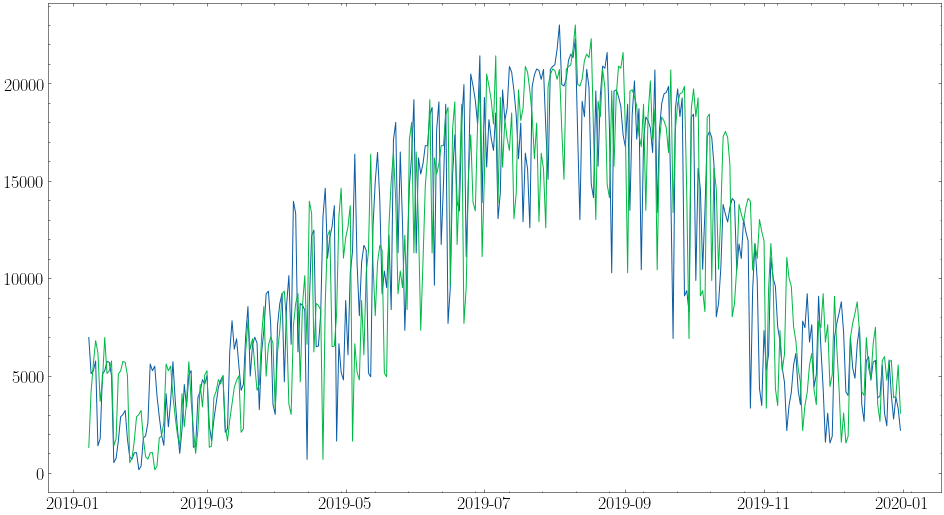
\includegraphics[width=16cm]{images/solution/predictions/baseline-predictions.png}
    \caption{Predicciones del modelo básico}
    \label{fig:baseline-predictions}
\end{figure}

Se puede observar que las predicciones son los mismos valores reales pero desplazados una semana. Una vez desarrollado este modelo, se han calculado las métricas que se muestran en la sección \ref{results} junto con el resto de los resultados de los otros modelos.
